\documentclass[hidelinks]{ctexart}

\usepackage{van-de-la-illinoise}
\usepackage[paper=b5paper,top=.3in,left=.9in,right=.9in,bottom=.3in]{geometry}
\usepackage{calc}
\pagenumbering{gobble}
\setlength{\parindent}{0pt}
\sisetup{inter-unit-product=\ensuremath{{}\cdot{}}}
\usepackage{van-le-trompe-loeil}
\usetikzlibrary{quotes,angles}
\usetikzlibrary{arrows.meta}
\usepackage{makecell}

\usepackage{stackengine}
\stackMath
\usepackage{scalerel}
\usepackage[outline]{contour}

\newdimen\indexlen
\def\newprobheader#1{%
\def\probindex{#1}
\setlength\indexlen{\widthof{\textbf{\probindex}}}
\hskip\dimexpr-\indexlen-1em\relax
\textbf{\probindex}\hskip1em\relax
}
\def\newprob#1{%
\newprobheader{#1}%
\def\newprob##1{%
\probsep%
\newprobheader{##1}%
}%
}
\def\probsep{\vskip1em\relax{\color{gray}\dotfill}\vskip1em\relax}

\newlength\thisletterwidth
\newlength\gletterwidth
\newcommand{\leftrightharpoonup}[1]{%
{\ooalign{$\scriptstyle\leftharpoonup$\cr%\kern\dimexpr\thisletterwidth-\gletterwidth\relax
$\scriptstyle\rightharpoonup$\cr}}\relax%
}
\def\tensor#1{\settowidth\thisletterwidth{$\mathbf{#1}$}\settowidth\gletterwidth{$\mathbf{g}$}\stackon[-0.1ex]{\mathbf{#1}}{\boldsymbol{\leftrightharpoonup{#1}}}  }
\def\onedot{$\mathsurround0pt\ldotp$}
\def\cddot{% two dots stacked vertically
  \mathbin{\vcenter{\baselineskip.67ex
    \hbox{\onedot}\hbox{\onedot}}%
}}%

    \tikzset{
    partial ellipse/.style args={#1:#2:#3}{
        insert path={+ (#1:#3) arc (#1:#2:#3)}
    }}

\begin{document}

\newprob{4.1 (1)}%
沿$+\+uz$传播, $\pare{\+ve_x,\+ve_y,\+uk}$构成右手系, $\+ve_x + i\+ve_y$是右旋基, 故为潘氏\underline{右旋}.\raisebox{-.4em}{\smash{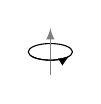
\begin{tikzpicture}
    \draw (0,0) ellipse (.8em and .3em);
    \draw[draw=gray,-latex] (0,-.3) -- (0,+.3);
    \draw[-latex] (0,0) [partial ellipse=210:330:.8em and .3em];
\end{tikzpicture}}}
\par
\newprobheader{(2)}%
沿$+\+uz$传播, $\pare{\+ve_x,\+ve_y,\+uk}$构成右手系, $\+ve_x - i\+ve_y$是左旋基, 故为潘氏\underline{左旋}.\raisebox{-.4em}{\smash{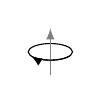
\begin{tikzpicture}
    \draw (0,0) ellipse (.8em and .3em);
    \draw[draw=gray,-latex] (0,-.3) -- (0,+.3);
    \draw[-latex] (0,0) [partial ellipse=330:210:.8em and .3em];
\end{tikzpicture}}}
\newprob{4.2}%
设三个区域$\+vE$如下:
\begin{center}
    \begin{tikzpicture}
        \draw (0,-1) -- (0,2);
        \draw (5,-1) -- (5,2);
        \draw[-latex] (-3.5,-1) -- (0,-1) node[below] {$0$} -- (5,-1) node[below] {$d$} -- (9.5,-1) node[below] {$z$};
        \draw[-latex] (-2,1.5) -- (-0.5,1.5) node[midway,above] {$k_1$};
        \draw[-latex] (-2,1.5) -- (-2,2.5) node[midway,left] {$E\+_I10_ e^{i\pare{k_1 z - \omega t}}$};
        \draw[-latex] (-0.5,0) -- (-2,0) node[midway,below] {$k_1$};
        \draw[-latex] (-0.5,0) -- (-0.5,1) node[midway,left] {$E\+_R10_ e^{i\pare{-k_1 z - \omega t}}$};
        %
        \draw[-latex] (3,1.5) -- (4.5,1.5) node[midway,above] {$k_2$};
        \draw[-latex] (3,1.5) -- (3,2.5) node[midway,left] {$E\+_I20_ e^{i\brac{k_2 \pare{z-d} - \omega t}}$};
        \draw[-latex] (4.5,0) -- (3,0) node[midway,below] {$k_2$};
        \draw[-latex] (4.5,0) -- (4.5,1) node[midway,left] {$E\+_R20_ e^{i\brac{-k_2 \pare{z-d} - \omega t}}$};
        %
        \draw[-latex] (8,0.5) -- (9.5,0.5) node[midway,above] {$k_3$};
        \draw[-latex] (8,0.5) -- (8,1.5) node[midway,left] {$E\+_T30_ e^{i\brac{k_3 \pare{z-d} - \omega t}}$};
    \end{tikzpicture}
\end{center}
则$\+vE_2$和$\+vE_3$的关系可直接由Fresnel公式得到,
    \[ \begin{cases}
        \displaystyle E\+_R20_ = \frac{n_2 - n_3}{2n_2}E\+_T30_, \\[.5em]
        \displaystyle E\+_I20_ = \frac{n_2 + n_3}{2n_2}E\+_T30_.
    \end{cases} \]
$\+vE_1$和$\+vE_2$的关系可通过列出$z=0$处的边界条件得到,
\begin{align*}&\begin{cases}
    E\+_R10_ + E\+_I10_ = E\+_I20_e^{-ik_2 d} + E\+_R20_ e^{ik_2 d}, \\
    \displaystyle \rec{n_2}\pare{E\+_R10_ - E\+_I10_} = \rec{n_1}\pare{E\+_R20_e^{-ik_2 d} - E\+_I20_e^{ik_2 d}}
\end{cases} \\ &\Rightarrow \begin{cases}
    \displaystyle E\+_R10_ = \frac{n_1\pare{E\+_R20_e^{-ik_2 d} + E\+_I20_e^{ik_2 d}} + n_2\pare{E\+_R20_e^{-ik_2 d} - E\+_I20_e^{ik_2 d}}}{2n_1}, \\[.5em]
    \displaystyle E\+_I10_ = \frac{n_1\pare{E\+_R20_e^{-ik_2 d} + E\+_I20_e^{ik_2 d}} - n_2\pare{E\+_R20_e^{-ik_2 d} - E\+_I20_e^{ik_2 d}}}{2n_1}.
\end{cases}\end{align*}
去掉共有的分母和$E\+_T30_$因子, 有
\begin{align*}
    E\+_R10_ &\propto n_1 \brac{\pare{n_2 - n_3}e^{ik_2 d} + \pare{n_2 + n_3}e^{-ik_2d}} + n_2 \brac{\pare{n_2-n_3}e^{ik_2 d} - \pare{n_2+n_3}e^{-ik_2 d}} \\
    & \propto \pare{n_1n_2 - n_2n_3}\cos k_2 d + i\pare{n_2^2 - n_1n_3} \sin k_2 d, \\
    E\+_I10_ &\propto n_1 \brac{\pare{n_2 - n_3}e^{ik_2 d} + \pare{n_2 + n_3}e^{-ik_2d}} - n_2 \brac{\pare{n_2-n_3}e^{ik_2 d} - \pare{n_2+n_3}e^{-ik_2 d}} \\
    & \propto \pare{n_1n_2 + n_2n_3}\cos k_2 d + i\pare{-n_1n_3 - n_2^2} \sin k_2 d, \\
    \abs{E\+_R10_}^2 & \propto n_2^2\pare{n_1 - n_3}^2\cos^2 k_2 d + \pare{n_2^2 - n_1n_3}^2 \sin^2 k_2 d, \\
    \abs{E\+_I10_}^2 & \propto n_2^2\pare{n_1 + n_3}^2\cos^2 k_2 d + \pare{n_2^2 + n_1n_3}^2 \sin^2 k_2 d, \\
    & \boxed{R = \frac{\abs{E\+_R10_}^2}{\abs{E\+_I10_}^2} = \frac{n_2^2\pare{n_1 - n_3}^2\cos^2 k_2 d + \pare{n_2^2 - n_1n_3}^2 \sin^2 k_2 d}{n_2^2\pare{n_1 + n_3}^2\cos^2 k_2 d + \pare{n_2^2 + n_1n_3}^2 \sin^2 k_2 d}.} \\
    \frac{E\+_T30_}{E\+_I10_} &= \frac{4n_2n_1}{n_1\brac{\pare{n_2-n_3} e^{-ik_2 d} + \pare{n_2+n_3}e^{ik_2 d}} - n_2\brac{\pare{n_2-n_3}e^{-ik_2 d} - \pare{n_2+n_3}e^{ik_2d}}} \\
    &= \frac{2n_2n_1}{\pare{n_1n_2 + n_2n_3}\cos k_2 d - i\pare{n_2^2 + n_1n_3}\sin k_2 d}. \\
    & \boxed{T = \frac{n_3 \abs{E\+_T30_}^2}{n_1 \abs{E\+_T10_}^2} = \frac{4n_2^2n_1n_3}{n_2^2\pare{n_1+n_3}^2\cos^2 k_2 d + \pare{n_2^2 + n_1n_3}^2\sin^2 k_2 d}.} \\
    R+T &= \frac{n_2^2\pare{n_1 - n_3}^2\cos^2 k_2 d + \pare{n_2^2 - n_1n_3}^2 \sin^2 k_2 d + 4n_2^2n_1n_3\pare{\cos^2 k_2 d + \sin^2 k_2 d}}{n_2^2\pare{n_1+n_3}^2\cos^2 k_2 d + \pare{n_2^2 + n_1n_3}^2\sin^2 k_2 d} = 1.
\end{align*}
\par
\newprobheader{(2)}%
欲使$R=0$, 须$n_2^2 - n_1n_3 = 0$, $\cos k_2 d = 0$, 当$n_3 = 1$时即
\[ \boxed{d = \pare{\frac{m}{2} + \rec{4}}\lambda_2,\quad n_2 = \sqrt{n_1},\quad m \in \+bN.} \]
\par
\newprobheader{转移矩阵}%
经过$n_2$介质的转移特性矩阵为(cf. \textit{Principles of Optics}, M. Born)
\[ M = \begin{pmatrix}
    \cos k_2 h & -iZ_2 \sin k_2 h \\
    \displaystyle -\frac{i}{Z_2}\sin k_2 h & \cos k_2 h
\end{pmatrix} = \begin{pmatrix}
    m_{11} & m_{12} \\
    m_{21} & m_{22}
\end{pmatrix},\quad \begin{pmatrix}
    E\+_10_ \\
    H\+_10_
\end{pmatrix} = M \begin{pmatrix}
    E\+_30_ \\
    H\+_30_
\end{pmatrix}. \]
从而
\begin{align*}&\begin{cases}
    \displaystyle E\+_I10_ + E\+_R10_ = \pare{m_{11} + \frac{m_{21}}{Z_3}}E\+_T30_, \\
    \displaystyle \rec{Z_1} \pare{E\+_I10_ - E\+_R10_} = \pare{m_{21} + \frac{m_{22}}{Z_3}}E\+_T30_
\end{cases}\\ &\Rightarrow \begin{cases}
    \displaystyle E\+_I10_ = \frac{n_2\pare{n_1+n_3}\cos hk_2 - i\pare{n_2^2 + n_1n_3}\sin hk_2}{2n_1n_2} E\+_T30_, \\[.5em]
    \displaystyle E\+_R10_ = \frac{n_2\pare{n_1-n_3}\cos hk_2 + i\pare{n_2^2 - n_1n_3}\sin hk_2}{2n_1n_2} E\+_T30_.
\end{cases}\end{align*}
可以得到相同的结果.
\newprob{4.3}%
$\+un \cdot \+vE\+_I_\vert_{z=0} + \+un\cdot \+vE\+_R_\vert_{z=0} = \+un\cdot\+vE\+_T_\vert_{z=0} = 0 \Rightarrow \+vE\+_R_ = \boxed{-E_0e^{-i\pare{kz+\omega t}}\+ve_x.}$\\
$\displaystyle \+v\kappa = \+vH\+_I_\times \+un\vert_{z=0} - \+vH\+_T_\times \+un\vert_{z=0} = \rec{Z_0}\pare{\+uk\times \+vE\+_I_ - \+uk\times \+vE\+_R_}\times \+un = \boxed{2E_0\sqrt{\frac{\epsilon_0}{\mu_0}}e^{-i\omega t}\+ve_x.}$
\newprob{4.4 (1)}%
$\+vS = \+vE\times \+vH = EH\+uk = \boxed{EH\pare{\cos\theta\+un + \sin\theta\+u\tau}.}$\\
$\+vS' = \+vE'\times \+vH' = E'H'\+uk' = \boxed{E'H'\pare{-\cos\theta\+un + \sin\theta\+u\tau}.}$\\
$\+vS'' = \+vE''\times \+vH'' = E''H''\+uk'' = \boxed{E''H''\pare{\cos\theta''\+un + \sin\theta''\+u\tau}.}$\\[-2.5em]
\begin{align*}
    &\phantom{=\ } \+un\cdot \+vS + \+un\cdot \+vS' - \+un\cdot \+vS'' \\
    &= \pare{EH-E'H'}\cos\theta - E''H''\cos\theta'' \\
    &\propto \sqrt{\epsilon_1}\pare{E^2-E'^2}\cos\theta - \sqrt{\epsilon_2}E''^2\cos\theta'' \\
    &\propto \sqrt{\epsilon_1}\brac{\pare{\sqrt{\epsilon_1}\cos\theta+\sqrt{\epsilon_2}\cos\theta''}^2 - \pare{\sqrt{\epsilon_1}\cos\theta-\sqrt{\epsilon_2}\cos\theta''}^2}\cos\theta - \sqrt{\epsilon_2}\pare{4\epsilon_1\cos\theta}\cos\theta'' \\
    &= 0.
\end{align*}
\par
\newprobheader{(2)}%
$\displaystyle R = \abs{\frac{E'}{E}}^2 = \boxed{\pare{\frac{\sqrt{\epsilon_1}\cos\theta - \sqrt{\epsilon_2}\cos\theta''}{\sqrt{\epsilon_1}\cos\theta + \sqrt{\epsilon_2}\cos\theta''}}^2.}$
\newprob{4.5}%
\vspace{-1.75\baselineskip}
\begin{flalign*}
    & \+un\cdot\pare{\+vE'\times \+vH + \+vE\times \+vH'} && \\
    & = \+un\cdot\pare{\+vE'\times\pare{\+vk\times \+vE} + \+vE\times\pare{\+vk'\times \+vE'}} && \\
    & = \+un\cdot\brac{\+vk\pare{\+vE'\cdot \+vE} - \pare{\+vE'\cdot \+vk}\+vE + \+vk'\pare{\+vE'\cdot \+vE} - \pare{\+vE\cdot \+vk'}\+vE'} && \\
    & = \+un\cdot\brac{2\+uk_x\pare{\+vE'\cdot \+vE} - 2\pare{\+vE'\cdot \+vk_n}\+vE + 2\pare{\+vE\cdot \+uk_n}\+vE'} \\
    &= \+un\cdot\brac{\pare{\+vE\cdot \+uk_n}\+vE' - \pare{\+vE'\cdot \+uk_n}\+vE} \\
    &= \pare{\+vE\cdot \+uk_n}\+vE'_n - \pare{\+vE'\cdot \+uk_n}\+vE_n \\
    &= 0.
\end{flalign*}
\hfill{\smash{\begin{tikzpicture}[xscale=0.8,yscale=0.8]
    \draw[-latex] (0,0) -- (1,2) node[midway,below,sloped] {$\+uk$};
    \draw[-latex] (1,2) -- (2,0) node[midway,above,sloped] {$\+uk'$};
    \draw[-latex] (1,2) -- (1,4.236) node[midway,left] {$\+un$};
    \draw[-latex] (0,0) -- (1,0) node[midway,below] {$\+uk_x$};
    \draw[-latex] (0,0) -- (0,2) node[above] {$\+uk_n$};
    \draw (0,0) ++ (64:0.6) arc (64:90:0.6) node [midway, above] {$\theta$};
    \draw[-latex] (0,0) -- (-1,2) node[above]{$\+vE^\parallel$};
    \draw[-latex] (-1,0) -- (0,0) node[midway,below]{$\+vE_x$};
    \draw[-latex] (-1,0) -- (-1,2) node[midway,left]{$\+vE_n$};
    \draw[-latex] (2,0) -- (4,1) node[above]{$\+vE'^\parallel$};
    \draw[-latex] (2,0) -- (4,0) node[midway,below]{$\+vE'_x$};
    \draw[-latex] (4,0) -- (4,1) node[midway,right]{$\+vE'_n$};
\end{tikzpicture}}}
\newprob{4.6}%
\vspace{-1.75\baselineskip}
\begin{flalign*}
    & \+un\+un\cddot \half\pare{\+vD\cdot \+vE' + \+vD'\cdot \+vE + \+vB\cdot \+vH' + \+vB'\cdot \+vH}\tensor{I} - \+un\+un\cddot \pare{\+vD\+vE' + \+vD'\+vE + \+vB\+vH' + \+vB'\+vH} && \\
    & \propto \frac{\+vE'\cdot \+vE}{2} - \pare{\+un\cdot \+vE'}\pare{\+un\cdot \+vE} + \frac{\pare{\+uk'\times \+vE'}\pare{\+uk\times \+vE}}{2} - \brac{\+un\cdot\pare{\+uk'\times \+vE'}}\brac{\+un\cdot\pare{\+uk\times \+vE}} && \\
    & = \frac{\+vE'\cdot \+vE}{2} - \pare{\+un\cdot \+vE'}\pare{\+un\cdot \+vE}\\
    &\phantom{=\ } + \frac{\pare{k_x^2 - k_n^2}\pare{\+vE'\cdot \+vE} + 4\pare{\+uk_n\cdot \+vE}\pare{\+uk_n\cdot \+vE'}}{2} - \brac{\+uk_x\cdot\pare{\+vE'\times \+un}}\brac{\+uk_x\cdot\pare{\+vE\times \+un}} && \\
    &= k_x^2\pare{\+vE'\cdot \+vE} - E'_nE_n + 2\cos^2\theta \pare{E'_zE_z} - \sin^2\theta E_yE'_y && \\
    &= \sin^2\theta \pare{E_xE'_x} + \cos^2\theta \pare{E_zE'_z} \\
    &= \sin^2\theta \pare{E_xE'_x} + \cos^2\theta \pare{-E_x\tan\theta}\pare{E'_x\tan\theta} \\
    &= 0.
\end{flalign*}
\vspace{-2\baselineskip}
\newprob{4.7}%
$\displaystyle \frac{\sigma}{\epsilon\omega} = \SI{3.60e7}{} \gg 1$.\\
$\displaystyle d = \rec{\alpha} \approx \sqrt{\frac{2}{\omega\mu\sigma}} = \boxed{\SI{71.2}{\meter}.}$
\newprob{4.8}%
$\displaystyle \frac{\sigma}{\epsilon\omega} = 0.288 < 1$. 不可使用良导体近似.\\
$\displaystyle \beta + i\alpha = \omega\sqrt{\mu \epsilon \pare{1+i\frac{\sigma}{\epsilon\omega}}} = \pare{374 + 52.8 i}\SI{}{\per\meter} \Rightarrow \rec{\alpha} = \boxed{\SI{1.90}{\centi\meter}.}$
\newprob{4.9}%
设导体内的场为$\displaystyle \+vE = \+vE_0 e^{-\+v\alpha\cdot \+vr}e^{i\pare{\+v\beta\cdot \+vr - \omega t}}$,
\begin{align*}
    \expc{P} &= \displaystyle \int_0^\infty \sigma\expc{\Re \+vE\cdot \Re \+vE}\,\rd{z} = \int_0^\infty \frac{\sigma}{2}\Re\pare{\+vE\cdot \+vE^*}\,\rd{z} \\
    &= \int_0^\infty \frac{\sigma}{2}E_0^2 e^{-2\alpha z}\,\rd{z} = \frac{\sigma}{4\alpha}E\+_0_^2.\\
    \expc{\+vS}\cdot \+vn &= \expc{\Re \+vE\vert_{z=0} \times \Re \+vH\vert_{z=0}} = \half \Re\pare{\+vE_0 \times \+vH_0}\cdot \+vn \\
    &= \rec{2\omega\mu}\Re\curb{\+vE_0\times \brac{\pare{\+v\beta-i\+v\alpha}\times \+vE_0^*}} \cdot \+vn \\
    &= \rec{2\omega\mu} \Re\curb{E_0^2\pare{\+v\beta - i\+v\alpha}\cdot \+vn} - \rec{2\mu\omega}\Re\curb{\brac{\+vE_0 \cdot \pare{\+v\beta - i\+v\alpha}}\brac{\+vE_0^*\cdot \+vn}} \\
    &= \rec{2\omega\mu\alpha} \pare{E_0^2\+v\beta\cdot \+v\alpha} - \rec{2\mu\omega\alpha}\Re\curb{\brac{\+vE_0 \cdot \pare{- 2i\+v\alpha}}\brac{\+vE_0^*\cdot \+v\alpha}} \\
    &=\rec{2\omega\mu\alpha} \pare{E_0^2\frac{\omega\mu\sigma}{2}} + \rec{\mu\omega\alpha}\Re\curb{i\pare{\+vE_0 \cdot {\+v\alpha}}\pare{\+vE_0^*\cdot \+v\alpha}} \\
    &= \frac{\sigma}{4\alpha}E_0^2.
\end{align*}
\newprob{Pr 1 (a)}%
$\displaystyle \+vE_1 = E_0\pare{\+ve_1 + i \+ve_2}e^{i\pare{kz - \omega t}}$,\quad $\displaystyle \+vE_2 = E_0 \pare{\+ve_1 + i\+ve_2}e^{i\pare{-kz-\omega t}}$. \\
$\displaystyle c\+vB_1 = E_0 \+uz\times\pare{\+ve_1 + i \+ve_2}e^{i\pare{kz - \omega t}}$,\quad $\displaystyle c\+vB_2 = -E_0 \+uz\times \pare{\+ve_1 + i\+ve_2}e^{i\pare{-kz-\omega t}}$. \\
$\displaystyle \+vE = \+vE_1 + \+vE_2 = 2E_0 \pare{\+ve_1 + i\+ve_2}\cos kz e^{-i\omega t}$\\
$\displaystyle \Rightarrow \boxed{\Re \+vE = 2E_0\cos kz\pare{\cos \omega t \+ve_1 + \sin \omega t \+ve_2}.}$\\
$\displaystyle c\+vB = c\+vB_1 + c\+vB_2 = 2E_0\pare{\+ve_1+i\+ve_2}\sin kz e^{-i\omega t}$ \\
$\displaystyle \Rightarrow \boxed{\Re \+vB = \frac{2E_0}{c}\sin kz\pare{\cos \omega t \+ve_1 + \sin \omega t \+ve_2}.}$
\par
\newprobheader{(b)}%
$\displaystyle \+vE_1 = E_0\pare{\+ve_1 + i \+ve_2}e^{i\pare{kz - \omega t}}$,\quad $\displaystyle \+vE_2 = E_0 \pare{\+ve_1 - i\+ve_2}e^{i\pare{-kz-\omega t}}$. \\
$\displaystyle c\+vB_1 = E_0 \+uz\times\pare{\+ve_1 + i \+ve_2}e^{i\pare{kz - \omega t}}$,\quad $\displaystyle c\+vB_2 = -E_0 \+uz\times \pare{\+ve_1 - i\+ve_2}e^{i\pare{-kz-\omega t}}$. \\
$\displaystyle \+vE = \+vE_1 + \+vE_2 = 2E_0 \pare{\cos kz\+ve_1 - \sin kz\+ve_2} e^{-i\omega t}$\\
$\displaystyle \Rightarrow \boxed{\Re \+vE = 2E_0 \pare{\cos kz\+ve_1 - \sin kz\+ve_2}\cos\omega t.}$\\
$\displaystyle c\+vB = c\+vB_1 + c\+vB_2 = \frac{2E_0}{i}\pare{\cos kz\+ve_1 - \sin kz\+ve_2} e^{-i\omega t}$ \\
$\displaystyle \Rightarrow \boxed{\Re \+vB = -\frac{2E_0}{c}\pare{\cos kz\+ve_1 - \sin kz\+ve_2}\sin\omega t.}$

\end{document}
